
%% Based on a TeXnicCenter-Template, which was
%% created by Christoph Börensen
%% and slightly modified by Tino Weinkauf.
%%%%%%%%%%%%%%%%%%%%%%%%%%%%%%%%%%%%%%%%%%%%%%%%%%%%%%%%%%%%%

\documentclass[a4paper,12pt]{article} %scrartcl This is a special class provided by the KOMA script, which does a lot of adjustments to adapt the standard LaTeX classes to european habits, change to [a4paper,12pt,twoside] for doublesided layout


%########################### Preferences #################################


% ******** vmargin settings *********
\usepackage{vmargin} %This give you full control over the used page arae, it maybe not the idea od Latex to do so, but I wanted to reduce to amount of white space on the page
\setpapersize{A4}
\setmargins{3.5cm}%			%linker Rand, left edge
		   {1.5cm}%     %oberer Rand, top edge
           {14.7cm}%		%Textbreite, text width
           {23.42cm}%   %Texthoehe, text hight
           {30pt}%			%Kopfzeilenhöhe, header hight
           {1cm}%   	  %Kopfzeilenabstand, header distance
           {0pt}%				%Fußzeilenhoehe footer hight
           {2cm}%    	  %Fusszeilenabstand, footer distance   
\setlength{\parindent}{0pt}  % keine Einrückung nach Absatz

% ********* Font definiton ************
\usepackage{t1enc} % as usual
\usepackage[latin1]{inputenc} % as usual
\usepackage{times}		
\usepackage{fancyhdr} %%%% define chead, cfoot
\usepackage[table]{xcolor}
\usepackage{longtable}
\usepackage{booktabs}
\usepackage{tabularx}
\usepackage{wallpaper}

% ********* for code listing ************
\usepackage{listings}  
\usepackage{color}
\definecolor{gray}{rgb}{0.4,0.4,0.4}
\definecolor{darkblue}{rgb}{0.0,0.0,0.6}
\definecolor{cyan}{rgb}{0.0,0.6,0.6}

\lstloadlanguages{XML}

%\lstdefinelanguage{XML}
%{
  %morestring=[b]",
  %morestring=[s]{>}{<},
%%  morecomment=[s]{<?}{?>},
  %morecomment=[s][\color{orange}]{<!--}{-->},
  %stringstyle=\color{black},
  %identifierstyle=\color{darkblue},
  %keywordstyle=\color{red},
  %morekeywords={xmlns,version,type,num},
	%showstringspaces=false,
%}


%\usepackage{mathptmx}  	%mathematical fonts for use with times, I encountered some problems using this package togather with pdftex, which I was not able to resolve

% ********* Graphics definition *******
%\usepackage[pdftex]{graphicx} % required to import graphic files
\usepackage{eso-pic} % these two are required to add the little picture on top of every page
\usepackage{everyshi} % these two are required to add the little picture on top of every page
\renewcommand{\floatpagefraction}{0.7} %default:0.5 allows two big pictures on one page
\usepackage{wrapfig}

%********** Enybeling Hyperlinks *******
\usepackage[pdfborder=000]{hyperref}% this enables jumping from a reference and table of content in the pdf file to its target

% ********* Table layout **************
\usepackage{booktabs}	  	%design of table, has an excellent documentation
\usepackage{multirow}     % multirows in tables

% ********* Caption Layout ************
\usepackage{ccaption} % allows special formating of the captions
\captionnamefont{\bf\footnotesize\sffamily} % defines the font of the caption name (e.g. Figure: or Table:)
\captiontitlefont{\footnotesize\sffamily} % defines the font of the caption text (same as above, but not bold)
\setlength{\abovecaptionskip}{0mm} %lowers the distace of captions to the figure

%\usepackage{scrpage2} %header and footer using the options for the KOMA script % defines cfoot chead; cannot be used at the same time as fancyhdr
\newcommand{\headfont}{\footnotesize\sffamily} % font for the header
\newcommand{\pnumfont}{\footnotesize\sffamily} % font for the pagenumbers

\usepackage{helvet}
\renewcommand{\familydefault}{\sfdefault}

% set colors for links and URLs
\usepackage{hyperref}
\hypersetup{
	colorlinks=true,
	linkcolor=black,
	urlcolor=blue}


%this defines the page style for the first pages: all empty
%\renewpagestyle{plain}%
%	{(\textwidth,0pt)%
%		{\hfill}{\hfill}{\hfill}%
%	(\textwidth,0pt)}%
%	{(\textwidth,0pt)%	
%		{\hfill}{\hfill}{\hfill}%
%	(\textwidth,0pt)}

% CUSTOM LISTING FORMAT

\lstdefinestyle{lststyle}{
%	belowcaptionskip=1\baselineskip,
	breaklines=true,
%	frame=L,
	xleftmargin=\parindent,
%	language=C,
	showstringspaces=false,
	basicstyle=\footnotesize\ttfamily,
%	keywordstyle=\bfseries\color{green!40!black},
%	commentstyle=\itshape\color{purple!40!black},
%	identifierstyle=\color{blue},
	stringstyle=\color{orange},
}
\lstset{escapechar=@,style=lststyle}
% JSON format
\usepackage{listings}
\usepackage{xcolor}

\colorlet{punct}{red!60!black}
\definecolor{background}{HTML}{EEEEEE}
\definecolor{delim}{RGB}{20,105,176}
\colorlet{numb}{magenta!60!black}

\lstdefinelanguage{json}{
	basicstyle=\small\ttfamily,
	numbers=left,
	numberstyle=\scriptsize,
	stepnumber=1,
	numbersep=8pt,
	showstringspaces=false,
	breaklines=true,
	frame=lines,
	backgroundcolor=\color{background},
	literate=
	*{0}{{{\color{numb}0}}}{1}
	{1}{{{\color{numb}1}}}{1}
	{2}{{{\color{numb}2}}}{1}
	{3}{{{\color{numb}3}}}{1}
	{4}{{{\color{numb}4}}}{1}
	{5}{{{\color{numb}5}}}{1}
	{6}{{{\color{numb}6}}}{1}
	{7}{{{\color{numb}7}}}{1}
	{8}{{{\color{numb}8}}}{1}
	{9}{{{\color{numb}9}}}{1}
	{:}{{{\color{punct}{:}}}}{1}
	{,}{{{\color{punct}{,}}}}{1}
	{\{}{{{\color{delim}{\{}}}}{1}
	{\}}{{{\color{delim}{\}}}}}{1}
	{[}{{{\color{delim}{[}}}}{1}
	{]}{{{\color{delim}{]}}}}{1},
}

\providecommand{\tightlist}{%
	\setlength{\itemsep}{0pt}\setlength{\parskip}{0pt}}

%----------------------------------------------------------------------------------------
%	BEGIN DOCUMENT
%----------------------------------------------------------------------------------------

\pagestyle{plain} % on headers or footers on the first page


%%%%%%%%%%%%%%%%%%%%%%%%%%%%%%%%%%%%%%%%%%%%%%%%%%%%%%%%%%%%%%%%%%%
 %%%%%%%%%%%%%         CHANGE VERSION NUMBER HERE    %%%%%%%%%%%
\newcommand{\version}{4.0.1}
 %%%%%%%%%%%%%%%%%%%%%%%%%%%%%%%%%%%%%%%%%%%%%%%%%%%%%%%%%%%%%%%
 %%%%%%%%%%%%%%%%%%%%%%%%%%%%%%%%%%%%%%%%%%%%%%%%%%%%%%%%%%%%%%%%%%%
 
\begin{document}

%----------------------------------------------------------------------------------------
%	TITLE PAGE
%----------------------------------------------------------------------------------------
\begin{titlepage}
	\centering
	{\scshape\Huge \textbf{ PRo3D \version} \par}
	{\scshape\Large User Manual\par}
	\vspace{1.cm}
	\includegraphics[width=1.0\textwidth]{pics/CoverPic.png}\par\vspace{1cm}		
	{\large Authors: \par
	Thomas Ortner, Laura Fritz, Rebecca Nowak}
	\vfill
	% Bottom of the page
	{Last Updated: \today\par}
\end{titlepage}

\newpage

\pagestyle{fancy} % now we want to have headers and footers

%----------------------------------------------------------------------------------------
%	Header and Footer
%----------------------------------------------------------------------------------------
\fancyhf{} %alle Kopf- und Fußzeilenfelder bereinigen
\fancyhead[R]{} %Kopfzeile rechts
\fancyhead[C]{} %zentrierte Kopfzeile
\fancyhead[L]{\includegraphics[height=30pt]{pics/logosSUM.png}} %Kopfzeile links
\renewcommand{\headrulewidth}{0.4pt} %obere Trennlinie

\fancyfoot[L]{{PRo3D \version}}

\fancyfoot[R]{\thepage} 
\renewcommand{\footrulewidth}{0.4pt} %untere Trennlinie

%----------------------------------------------------------------------------------------
%	Change Records 
%----------------------------------------------------------------------------------------

%\begin{table}[h]
	%\centering
	%
		%\caption{\textbf{Change Records}}
		%\label{tab:changeRecs}
		%
		%\rowcolors{1}{lightgray}{white}
%
		%\begin{tabular}{c c p{7cm} p{3cm}}
			%\textbf{ISSUE} & \textbf{DATE} & \textbf{§ CHANGE RECORDS} & \textbf{AUTHOR} \\
			%\hline
			%1.0 & 2018-01-23 & Initial Version & Ortner, Fritz
		%\end{tabular}
%
%\end{table}

\newpage

%----------------------------------------------------------------------------------------
%	Table of Contents + List of Figures
%----------------------------------------------------------------------------------------
\tableofcontents
%\listoffigures

\newpage
%----------------------------------------------------------------------------------------
%	Section: Introduction
%----------------------------------------------------------------------------------------
\include{Introduction}
%----------------------------------------------------------------------------------------
%	Section: Start
%----------------------------------------------------------------------------------------
\include{Start}
%----------------------------------------------------------------------------------------
%	Section: Viewer Actions
%----------------------------------------------------------------------------------------
\include{ViewerActions}
%----------------------------------------------------------------------------------------
%	Section: Viewer Features
%----------------------------------------------------------------------------------------
%----------------------------------------------------------------------------------------
%	Section: Viewer Features
%----------------------------------------------------------------------------------------
\section{Viewer Features}

\begin{figure}[h]
    	\centering
    		\includegraphics[width=1\textwidth]{pics/SurfacesAI.png}
    	\caption[Viewer Features]{There are pages (right) for each feature in the viewer.}
    	\label{fig:featureMenu}
   \end{figure}
	
The feature pages show a list of the respective features, the properties of the selected feature from this list, and some actions for this feature.
For surfaces, annotations, and bookmarks it is possible to group them, as described in Section~\ref{sec:grouping}.
%----------------------------------------------------------------------------------------
%	SubSection: Surfaces
%----------------------------------------------------------------------------------------
\subsection{Surfaces}
\label{sec:surfaces}

The listing shows all surfaces in the scene. You can classify them in any group and subgroup layers, described in Section~\ref{sec:grouping}.
You can select a surface by clicking on the surface's name, which turns its color to green. Or you can set ``PickSurface'' in the actions menu (Figure~\ref{fig:Interactions}), press CTRL+LMB and pick the surface in the main view. Then you can see the surface's properties in the properties panel and use the actions in the actions panel. 
It is also possible to select multiple surfaces by clicking the square icon in front of each surface. The selected surfaces have a green square in the list. The multiselection is used to move one ore more surfaces from one group to the active group.
Under the surface's name is a little menu:
\begin{itemize}
	\item \textit{FlyTo}: A click on the button triggers a FlyTo animation.
	\item \textit{openFolder}: Opens the folder where the scene file resides.	
	\item \textit{Cloud}: Creates new kd-tree files.	
	%\item \textit{portable}: This creates a folder hierarchy as used in the old viewer version. A scene file is created and the surfaces are
  %copied to the surface folder.
	\item \textit{Toggle Visible}: Toggles the surface visible/invisible.	
	\item \textit{Toggle IsActice}: You can only pick on active surfaces (explore center, annotations, ...).
	
\end{itemize}

\begin{figure}[h]
    	\centering
    		\includegraphics[width=1\textwidth]{pics/SurfaceTranslation.png}
    	\caption[Surface Translation]{Translation of the selected surface along the axes of the coordinate system.}
    	\label{fig:surfaceTranslation}
   \end{figure}

For each selected surface there are several panels as shown in Figure~\ref{fig:featureMenu} A to E. 

In the surface properties panel (Figure~\ref{fig:featureMenu} A) some adjustments are possible:
\begin{itemize}
	\item \textit{Name}: The surface's name. You can change it in the text field and press ``enter''.
	\item \textit{Visible}: The surface is visible (checked) or not (unchecked).
	\item \textit{Active}: The surface is active (checked) or not (unchecked). You can only pick on active surfaces.
	\item \textit{Priority}:  Often multiple surfaces are available for a certain area on the planet surface. These surfaces represent the same piece of ground and typically overlap. This parameter allows you to assign a priority to a surface to tell the graphics card which surface should be rendered in front. Lower numbers mean a higher priority in rendering, with 0 being the highest priority. You can also give the highest priority surface a ranking of, for instance, 0.1 (= 10cm) to make annotations more visible. The priority can be dynamically changed via the surface properties so you can try out what works best.
	\item \textit{Quality}: 
	\item \textit{TriangleFilter}: Excludes triangles with edges bigger than the entered value.
	\item \textit{Scale}: 
	\item \textit{FillMode}: You can switch between solid/ wireframe/ point rendering of the geometry.
	\item \textit{Scalars}: Select an attribute layer.
	\item \textit{Textures}: Select a texture layer.
	\item \textit{Cull Faces}:
	\item \textit{Set Homeposition}: You set a new camera position for FlyTo.
\end{itemize}

The surfaces actions (Figure~\ref{fig:featureMenu} B) are described in Section~\ref{sec:leafActions}. \\


You can translate the surface along the north-, east and up axis of the coordinate system, described in Section~\ref{sec:placeCS}. And you can rotate the surface around the up vector of the coordinate system. The Translation panel is shown in Figure~\ref{fig:featureMenu} B and Figure~\ref{fig:surfaceTranslation}. \\

\begin{center}
\colorbox{red}{\parbox{1.0\textwidth}{NOTE: Translation and Rotation only work for surfaces. Annotations, Rovers, the Coordinate System, etc. will NOT move with the surface. You have to transform the surface first!}}
\end{center}

\begin{figure}[h]
    	\centering
    		\includegraphics[width=1\textwidth]{pics/SurfaceColorCorrection.png}
    	\caption[Surface Color Correction]{Contrast-, brightness- and color filters applied on the selected surface.}
    	\label{fig:surfaceColorCorrection}
   \end{figure}

You can apply different color correction filters on the selected surface	(Figure~\ref{fig:surfaceColorCorrection}). \\

\begin{figure}[h]
    	\centering
    		\includegraphics[width=1\textwidth]{pics/SurfaceColorLegend.png}
    	\caption[Surface Color Legend]{A height map visualized by false color mapping.}
    	\label{fig:surfaceColorLegend}
   \end{figure}
	
Within the effort of including more and more meta data for a surface we included the so-called SurfaceAttributes (see Figure~\ref{fig:surfaceColorLegend}),
which are specified in an .opcx file carrying the name of the respective surface.
For now, these surface attributes mainly contain additional layers, which can either be a texture layer or an attribute layer.
Texture layers are just alternative texture maps that can be mapped onto the surface, such as images from different filters or even sensors (spectral image). 
Attribute maps on the other hand present an additional value for each position of a surface. 
If a surface has an .opcx file attached its layers are listed and can be selected in the \textit{Scalars} and the \textit{Textures} combo boxes as part of the surface's property control (Figure~\ref{fig:featureMenu}). 
In the Scalars ColorLegend panel, the color legend can be adjusted (Figure~\ref{fig:surfaceColorLegend}).

%----------------------------------------------------------------------------------------
%	SubSection: Annotations
%----------------------------------------------------------------------------------------
\newpage
\subsection{Annotations}
\label{sec:annotations}

\begin{figure}[h]
    	\centering
    		\includegraphics[width=1\textwidth]{pics/AnnotationsAI.png}
    	\caption[Viewer Features Annotations]{The annotations page.}
    	\label{fig:annoProps}
   \end{figure}
	
The listing shows all annotations in the scene. You can classify them in any group and subgroup layers, described in Section~\ref{sec:grouping}.
You can select an annotation by clicking on the annotation's name, which turns its color to green. Or you can set ``PickAnnotation'' in the actions menu (Figure~\ref{fig:Interactions}), press CTRL+LMB and pick the annotation in the main view. Then you can see the annotation's properties in the properties panel and use the actions in the actions panel. 
It is also possible to select multiple annotations by clicking the square icon in front of each annotation. The selected annotations have a green square in the list. The multiselection is used to move one ore more annotations from one group to the active group.\\
Under the annotation's name is a little menu:
\begin{itemize}
  \item \textit{Toggle}: Toggles the annotation visible/invisible.
	\item \textit{FlyTo}: A click on the button triggers a FlyTo animation.
\end{itemize}

For each selected annotation there are several panels as shown in Figure~\ref{fig:annoProps} A to E. 

The properties of the selected annotation (click on annotation's name) are shown in Figure~\ref{fig:annoProps} A. There you can get information and change some of the settings:
\begin{itemize}
	\item \textit{Geometry}: Shows the annotation mode (described in Section~\ref{sec:drawAnnotation}). This is not changeable retrospectively.
	\item \textit{Projection}: Shows the projection which determines the direction of the picking ray (described in Section~\ref{sec:drawAnnotation}, shown in Figure~\ref{fig:projection}). This is not changeable retrospectively.
	\item \textit{Semantic}: 
	\item \textit{Thickness}: You can change the annotation's line thickness.
	\item \textit{Color}: You can change the annotation's color.
	\item \textit{Text}: You can append a note. Write in the text field and press ``Enter''. The note will appear next to the annotation in the viewer. 
	\item \textit{TextSize}: You can change the textsize.
	\item \textit{Visible}: The annotation is visible (checked) or not (unchecked).
	\item \textit{ShowDnS}: For each annotation with more than three picking points Dip and Strike information (Section~\ref{sec:drawAnnotation}) is available. The DnS is visible (checked) or not (unchecked).
\end{itemize}

The annotations actions (Figure~\ref{fig:annoProps} B) are described in Section~\ref{sec:leafActions}.\\

The measurements tab (Figure~\ref{fig:annoProps} C) contains some information:
\begin{itemize}
	\item \textit{Position}: Shows the position (only for point annotations).
	\item \textit{PrintPosition}: Prints the position in the console window.
	\item \textit{Height}:  The height between the annotation's start and end point.
	\item \textit{HeightDelta}: The height difference between the highest and lowest point of the projected line.
	\item \textit{AvgAltitude}: The average altitude.
	\item \textit{Length}: The sum of direct distances between the picking points.
	\item \textit{WayLength}: The sum of projected distances between the picking points.
	\item \textit{Bearing}: The annotation's bearing.
	\item \textit{Slope}: The annotation's slope.
	\item \textit{Vertical Distance}: The vertical distance between the annotation's start and end point in relation to the up vector of the coordinate system.
	\item \textit{Horizontal Distance}: The horizontal distance between the annotation's start and end point in relation to the north- and right vector of the coordinate system.
\end{itemize}

\begin{figure}[h]
    	\centering
    		\includegraphics[width=1\textwidth]{pics/DnsAI.png}
    	\caption[Viewer Features DnSColorLegend]{Colorcoding of the Dip\&Strike annotations according to their dipping angles.}
    	\label{fig:dnSColorLegend}
   \end{figure}
	
Measurements for the dip and strike annotations are shown in the Dip\&Strike tab (Figure~\ref{fig:annoProps} D and Figure~\ref{fig:dnSColorLegend} D).\\

The color coding of the DnS annotation's discs and arrows is specified by the dipping angle. The color legend's parameters can be adjusted in the
Dip\&Strike ColorLegend tab shown in Figure~\ref{fig:dnSColorLegend} E.

%----------------------------------------------------------------------------------------Import AnnotationGroups
%\subsubsection{Import Annotations from old viewer versions} 
%
%To import annotations from old scene files click the ``browse'' button in the \textbf{ImportAnnotationGroups} section in the Scene Menu (Figure~\ref{fig:StartMenu}). This opens a folder browser dialog, where you can select an old scene file an click ''Open''.
%The annotations are loaded in the same group hierarchy to the ``root'' group.


%----------------------------------------------------------------------------------------
%	SubSection: ViewPlanner
%----------------------------------------------------------------------------------------
%\subsection{ViewPlanner}
%\label{sec:viewPlanner}

%----------------------------------------------------------------------------------------
%	SubSection: Bookmarks
%----------------------------------------------------------------------------------------
\subsection{Bookmarks}
\label{sec:bookmarks}

%\begin{figure}[h]
    	%\centering
    		%\includegraphics[width=0.5\textwidth]{pics/bookmarks.png}
    	%\caption[Viewer Features Bookmarks]{The bookmarks tab.}
    	%\label{fig:bookmarks}
   %\end{figure}
	
Bookmarks enable the user to record a certain camera viewpoint.
To add a new bookmark click the ``+'' button on top of the page. The new bookmark is added to the active group in the bookmarks listing.
To view the bookmark's properties and actions click on the bookmark's name. Clicking the ``house'' button beside the bookmark's name triggers a FlyTo. For multiselection click on the bookmark's square icons.

%----------------------------------------------------------------------------------------
%	SubSection: Bookmarks
%----------------------------------------------------------------------------------------
\subsection{Sequenced Bookmarks}
\label{sec:sequenced_bookmarks}

Sequenced bookmarks can be used to create, view, and record camera flight paths between bookmarks (Figure \ref{fig:seqBookmarks}). Properties like visibility of surfaces, annotations, and scale bars (the \emph{scene state}) are also recorded with bookmarks, and applied during animations.

\begin{figure}[h]
	\centering
	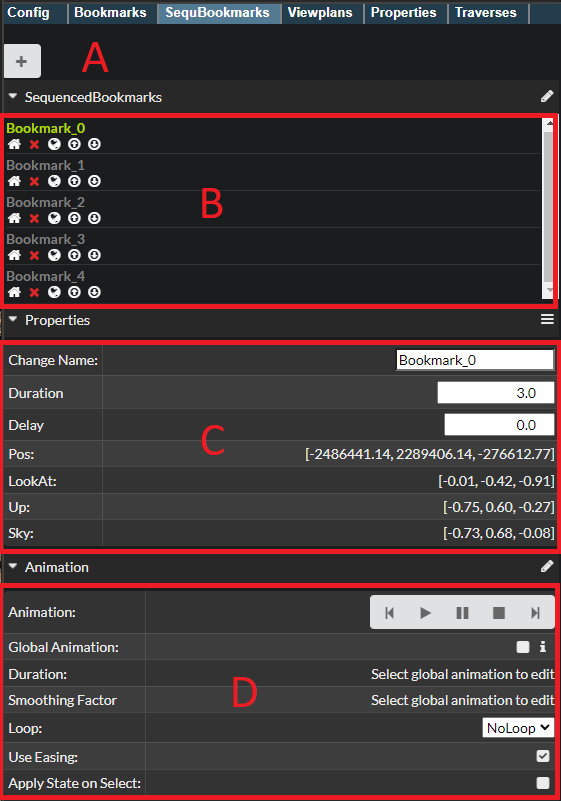
\includegraphics[width=0.5\textwidth]{pics/SequencedBookmarks_tabUpper.PNG}
	\caption[Viewer Features Bookmarks]{The sequenced bookmarks tab.}
	\label{fig:seqBookmarks}
\end{figure}

The scene state includes properties of surfaces, annotations and scale bars. It also includes general viewer settings in the \emph{Config} tab. 

Add bookmarks by clicking on the button with the plus icon at the top (A).

\begin{figure}[h]
	\centering
	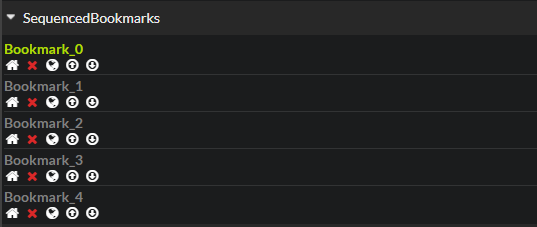
\includegraphics[width=0.8\textwidth]{pics/SequencedBookmarks_list.png}
	\caption[Viewer Features Bookmarks]{The list of all sequenced bookmarks.}
	\label{fig:seqBookmarks_list}
\end{figure}

In the list of bookmarks (B, Figure \ref{fig:seqBookmarks_list}) you can (from left to right) move the camera to the bookmark, delete the bookmark, update the scene state, and move the bookmark up and down in the list. Clicking on the label of a bookmark selects it. The selected bookmark is highlighted in green.

Updating the scene state for an annotation does not update its camera view.

\begin{figure}[h]
	\centering
	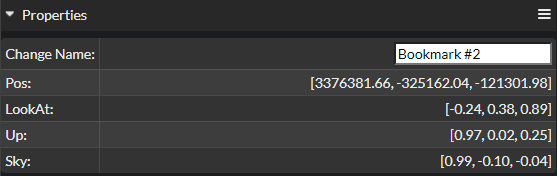
\includegraphics[width=0.8\textwidth]{pics/SequencedBookmarks_properties.png}
	\caption[Viewer Features Bookmarks]{The properties of the selected bookmark.}
	\label{fig:seqBookmarks_properties}
\end{figure}

You can find the properties of the selected bookmark (Figure \ref{fig:seqBookmarks_properties}) below the list of bookmarks (C). Here you can change the bookmark's name.

For each bookmark, you can set two values. The \emph{duration} is the amount of time it takes the camera to move from the previous bookmark to this bookmark. The \emph{delay} determines how long the camera pauses at the bookmark before moving to the next one.

\begin{figure}[h]
	\centering
	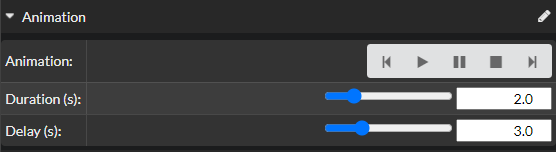
\includegraphics[width=0.8\textwidth]{pics/SequencedBookmarks_animation.png}
	\caption[Viewer Animation]{Animation settings.}
	\label{fig:SequencedBookmarks_animation}
\end{figure}

You can animate the camera according to the list of bookmarks by clicking the play button in the \emph{Animation} section (D). The animation control buttons from left to right: Move to previous bookmark, start camera animation along all bookmarks, pause camera animation, stop camera animation, move camera to next bookmark.

Selecting the checkbox \emph{global animation} has the following effects: 

\begin{itemize}
	\item A spline is used to travel a path along all bookmarks. The smoothing factor determines how smooth the path is. A value closer to zero means that the path hits individual bookmarks more precisely while a larger in general means a smoother path.
	\item The duration is set for the whole animation and cannot be set for individual bookmarks.
	\item The delay for individual bookmarks can not be used.
\end{itemize}

If there are large changes in the scene (and depending on hardware) the animation might not be entirely smooth when proceeding to a new bookmark.

There are three settings for looping: No loop, mirror, and repeat.

If the checkbox \emph{use easing} is selected, the camera animation speeds up in the beginning, and slows down at the end. When global animation is selected, easing is used at the beginning and the end of the whole path. When it is not selected, easing is used for each bookmark.


%\begin{figure}[h]
%	\centering
%	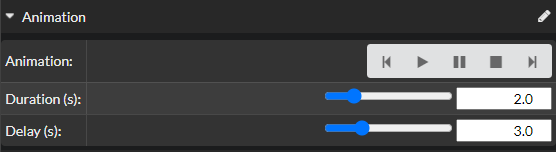
\includegraphics[width=0.8\textwidth]{pics/SequencedBookmarks_animation.png}
%	\caption[Viewer Features Bookmarks]{The animation controls. Buttons from left to right: Move to previous bookmark, start camera animation along all bookmarks, pause camera animation, stop camera animation, move camera to next bookmark.}
%	\label{fig:seqBookmarks_animation}
%\end{figure}


\begin{figure}[h]
	\centering
	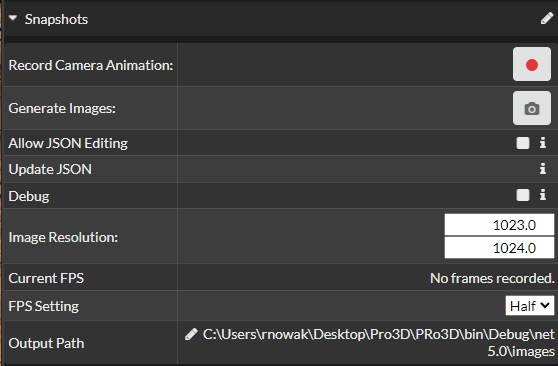
\includegraphics[width=0.8\textwidth]{pics/SequencedBookmarks_tabSnapshots.png}
	\caption[Viewer Features Bookmarks]{Creating images from sequenced bookmarks. Record camera animations as JSON snapshot files (red record button) and start generating images (camera button).}
	\label{fig:SequencedBookmarks_tabSnapshots.PNG}
\end{figure}

In the \emph{snapshots} section (Figure \ref{fig:SequencedBookmarks_tabSnapshots}) you can record camera animations. The red button changes to a \emph{stop} button when you start recording. If you now use the animation controls (D) to animate the camera, the camera movement is recorded. Once you click on the red stop button, a JSON file with the recorded camera animation is saved into the output folder specified in the \emph{Snapshots} section (E). To start rendering images with the saved file, click on the button with the camera icon next to the red record button. PRo3D will start rendering the images in the background.

The following settings are available:
\begin{itemize}
	\item \textbf{\emph{Allow JSON Editing}} There are more options for generating images you can use if you edit the JSON file PRo3D creates (see section \ref{sec:snapshots}). Select this option if you want to edit additional properties in the JSON file (like the field of view) manually. If this option is selected, the JSON file is NOT regenerated when clicking on the \emph{Generate Images} button. This means that settings changed after recording will not be taken into account. Click on the \emph{Update} button if you want to update the JSON file, but be aware that all manual changes will be overwritten. Make sure to backup a JSON file once you have changed it manually, as PRo3D will write over it as soon as you record a new sequence. You can also start the generation process via the command line (Section \ref{sec:CLI}) using an old JSON file. 
	\item \textbf{\emph{Update JSON}} Only available if \emph{Allow JSON Editing} is selected. Updates the JSON file with the current settings. All manual changes to the JSON file are overwritten. 
	\item \textbf{\emph{Image Resolution}} Resolution of output images. Larger images take longer to render.
	\item \textbf{\emph{Current FPS}} Once an animation sequence has been recorded, the FPS of that sequence are displayed here.
	\item \textbf{\emph{FPS Setting}} You can select full or half FPS, the actual FPS depend on the value displayed as \emph{Current FPS}. 
	\item \textbf{\emph{Output Path}} The path where the rendered images will be saved. Click on the path to change it.
\end{itemize}

To record an animation sequence follow these steps (the letters in parentheses refer to figure \ref{fig:seqBookmarks}):

\begin{enumerate}
	\item Add some sequenced bookmarks at different locations using the + button (A).
	\item Set delay and duration to your liking (C). Press play to test your settings (D).
	\item Set image resolution and other snapshot settings (E).
	\item Click on the red record button in the snapshots section (E).
	\item Click on play to start the animation (D).
	\item Wait until the animation is finished.
	\item Click on the red stop button in the Snapshots section (E).
	\item Click on the button with the camera icon (E, \emph{Generate Images}).
\end{enumerate}
%----------------------------------------------------------------------------------------
%	SubSection: Viewer Configuration
%----------------------------------------------------------------------------------------
\subsection{Viewer Configuration}
\label{sec:config}

To edit the viewer properties, select the ``Config'' page.

%----------------------------------------------------------------------------------------Viewer Config
\subsubsection{ViewerConfig} 

A set of major viewer properties can be adjusted:
\begin{itemize}
	\item \textit{Near/Far Plane}: The near- and the far clipping plane are automatically adjusted according to the data to be rendered. The set values are shown in the config panel and can be adjusted afterwards. 
	\item \textit{Navigation Sensitivity}: The navigation sensitivity can also be adjusted by PageUp and PageDown keys. 
	\item \textit{Arrow Length/Thickness}: The arrow length and thickness is set for up- and north vectors, dip and strike vectors and the up- and lookAt vectors in the rover view planner. 
	\item \textit{D+S Plane Size}: The dip and strike measurements plane size, described in Section~\ref{sec:drawAnnotation}
 (Figure~\ref{fig:drawAnnotations}).
	\item \textit{Min/Max Dipping Angle}: The dip and strike measurements dipping angle range. The dipping angle is coded into the color of the disc and arrow of a measurement (Figure~\ref{fig:drawAnnotations}).
	\item \textit{Lod Colors}: The different levels of detail of the surface geometry can be colored in different shades of red.
			This helps to evaluate the export of OPC data.
\end{itemize}

%----------------------------------------------------------------------------------------Coordinate System
\subsubsection{Coordinate System} 

The coordinate system menu shows the position, Up- and North Vector of the coordinate system described in Section~\ref{sec:placeCS}, shown in Figure~\ref{fig:coordinateSystem}.
The Up- and the North Vector are used for the projection measurements (Figure~\ref{fig:drawAnnotations}). Initially the Up Vector's direction is set in the positive z-direction and the North Vector's in the positive y-direction. But you can manipulate the Up Vector manually for different data. Both vectors are computed automatically with picking of a new position for the coordinate system. The north vector is further relevant for bearing measurements. % and the rover placement in the View Planner (see Section 4.6). 

%----------------------------------------------------------------------------------------Camera
\subsubsection{Camera} 

The Camera submenu shows the Location, Forward- and Sky vector of the main camera.


\subsubsection{Frustum}

In this menu the frustum can be adjusted.

\subsubsection{Screenshots}

This menu can be used to create screenshots of the current scene. Click on the button with the camera icon (left) to create a screenshot. Click on the button with the folder icon (right) to open the folder where screenshots are saved. Width and height can be specified in pixels. The output format can be selected as PNG or JPG. Screenshots are saved as \texttt{img} with a number suffix. 

\begin{figure}[h]
	\centering
	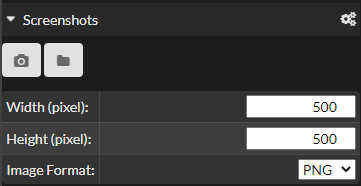
\includegraphics[width=0.6\textwidth]{pics/screenshots.PNG}
	\caption[View Planner]{The screenshots menu. Click on the button with the camera icon (left) to create a screenshot. Click on the button with the folder icon (right) to open the folder where screenshots are saved.}
	\label{fig:screenshots}
\end{figure}



%----------------------------------------------------------------------------------------
%	SubSection: Grouping
%----------------------------------------------------------------------------------------
\subsection{Grouping}
\label{sec:grouping}

%\begin{figure}[h]
    	%\centering
    		%\includegraphics[width=0.5\textwidth]{pics/GroupsProperties.png}
    	%\caption[Viewer Features]{The group properties and actions.}
    	%\label{fig:groupProps}
   %\end{figure}

Grouping is possible for surfaces, annotations and bookmarks.
The ``root'' group is the highest level where you can add leafs and subgroups.
Each group has a context menu:
\begin{itemize}
	\item \textit{Set Active}: The active group gets the new leaf. Per default the ``root'' is active.
	\item \textit{Add Group}: Adds a new and empty subgroup.
	\item \textit{Toggle Group}: Sets all leafs in this group and its subgroups invisible.
\end{itemize}

%----------------------------------------------------------------------------------------Group actions
\subsubsection{Group Actions}
\label{sec:groupActions}

\begin{itemize}
	\item \textit{Remove}: Removes the group with all its leafs and subgroups.
	\item \textit{Clear}: Removes all leafs and subgroups from group but retains the empty group. 
	\item \textit{Selection: Move}: Moves all selected leafs (green squares) to the active group.
	\item \textit{Selection: Clear}: Clears the selection (the leafs were not removed).
\end{itemize}
	
%----------------------------------------------------------------------------------------Leaf actions
\subsubsection{Leaf Actions}
\label{sec:leafActions}

\begin{itemize}
	\item \textit{Remove}: Removes the leaf.
	\item \textit{Selection: Move}: Moves all selected leafs (green squares) to the active group.
	\item \textit{Selection: Clear}: Clears the selection (the leafs were not removed).
\end{itemize}

%----------------------------------------------------------------------------------------
%	SubSection: ViewPlanner
%----------------------------------------------------------------------------------------
\newpage
\subsection{View Planner}
\label{sec:viewplanner}

\begin{figure}[h]
    	\centering
    		\includegraphics[width=1\textwidth]{pics/ViewPlanner1.png}
    	\caption[View Planner]{The view planner. The rover is placed on the surface in the main view (left). All rovers in the scene are listed in the ViewPlanner tab (right).}
    	\label{fig:viewPlanner}
   \end{figure}
To use the View Planner make sure that a \textbf{rover.xml} file is in the \textbf{\path{Release\InstrumentStuff}} folder. Then you can place one or more rover into your scene.
Therefore set ``PlaceRover'' in the actions menu (Figure~\ref{fig:viewPlanner} A), select a rover model in the rover menu (Figure~\ref{fig:viewPlanner} B), press CTRL+LMB and pick two points on the surface in the main view. The first point (green) is the position and the second point (yellow) the viewing direction of the rover. In the ViewPlanner tab is a listing that shows all ViewPlans in the scene (Figure~\ref{fig:viewPlanner} C). There is a little menu beside each ViewPlan shown in Figure~\ref{fig:viewPlanner} D:
\begin{itemize}
	\item FlyTo: clicking on the ``house button'' triggers an animation to the camera position from where the rover placement happened.
	\item (In)Visible: switch the rover to visible\textbackslash invisible.
	\item Remove: clicking on the red ``x'' removes the View Plan from the list and the view.
\end{itemize}
Select a view plan by clicking on the square icon in front of it to adjust it's properties:
\begin{itemize}
	\item ChangeVPName: change the name and press the enter button.
	\item Name: shows the rover's name.
	\item Instrument: select an instrument (camera) from the list (Figure~\ref{fig:viewPlanner} E).
\end{itemize}
\begin{figure}[h]
    	\centering
    		\includegraphics[width=1\textwidth]{pics/ViewPlannerGuiAi.png}
    	\caption[View PlannerGui]{The footprint for the selected camera is shown in light gray on the surface in the main view. In the properties panel (right) you can adjust the rover and camera parameters.}
    	\label{fig:viewPlannerGui}
   \end{figure}
When a camera is selected you can change the instrument parameters as shown in Figure~\ref{fig:viewPlannerGui} A:
\begin{itemize}
	\item Sensor (px): the image size in pixel.
	\item Focal (mm): the focal length of the camera sensor (zoom).
\end{itemize}
You can also change the rover's pan- and tilt axis (in degree) (Figure~\ref{fig:viewPlannerGui} B).
In the main view the footprint of the selected camera is shown in light gray. For the footprint there are following settings:
\begin{itemize}
	\item show footprint: you can enable\textbackslash disable the footprint in the main view.
	\item export footprint: you get one screenshot from the main view, one from the instrument view (Figure~\ref{fig:instView}) and a \textbf{*.svx} file with diverse meta information.
	\item open footprint folder: opens the folder with the screenshots and the meta file.
\end{itemize}
\begin{figure}[h]
    	\centering
    		\includegraphics[width=1\textwidth]{pics/InstrumentView.png}
    	\caption[Instrument View]{The instrument view (right) shows the instrument's camera view.}
    	\label{fig:instView}
   \end{figure}
%----------------------------------------------------------------------------------------
%	Section: Minerva
%----------------------------------------------------------------------------------------
\include{Minerva}
%----------------------------------------------------------------------------------------
%	Section: Command Line Interface
%----------------------------------------------------------------------------------------
%----------------------------------------------------------------------------------------
%	Section: PRo3D Command Line Interface
%----------------------------------------------------------------------------------------
\section{PRo3D Command Line Interface}

The PRo3D SnapshotViewer can produce rendered images in a batch process via the command line. For this process, \emph{snapshot files} are used. They are in the JSON format, and contain transformations for each rendered image. There are two types of snapshot files: One type that only transforms camera parameters, and another that can be used to transform surfaces as well. This section describes the format of these files, and how they can be used with PRo3D to render an arbitrary number of images.

%----------------------------------------------------------------------------------------
%	SubSection: Start Command Line
%----------------------------------------------------------------------------------------
\subsection{PRo3D Snapshot Files}
\label{sec:snapshots}

Snapshot files have the JSON format, and need to follow a distinct scheme to be usable with PRo3D. Examples can be found in section \ref{cl:examples}.

Field of view and resolution of the resulting image are only specified once, at the beginning of the file. The parameter \textit{snapshots} contains one entry for each output image. Table  \ref{table:json} lists all available parameters of the format.

 \begin{center}
	\begin{table}
		\begin{tabular}{p{0.2\linewidth} p{0.12\linewidth} p{0.6\linewidth}}
		\textbf{Parameter}         & 		 & \textbf{Comment} \\
		\midrule
		fieldOfView 	  & required &\\ 
		resolution 		  & required & resolution of the output image\\  
		snapshots 		  & required & each entry in this list will result in one output image\\    
		filename 		  & required & name of the output file\\ 
		view 			  & required & camera parameters \\  
		forward           & required & forward vector of the camera\\
		location          & required & location of the camera\\
		up                & required & up vector of the camera\\
		surfaceUpdates    & optional & \\    		
		opcname 		  & required & name of the surface to be transformed\\    		
		trafo 			  & optional & transformation to be applied to the surface\\    		
		visible 		  & optional & visibility of the surface \\  			
		\specialrule{\lightrulewidth}{1.0pt}{4.0pt}				
	\end{tabular} 
	\label{table:json}
	\caption{Available parameters for a PRo3D Snapshot file}
	\end{table}
\end{center}



%----------------------------------------------------------------------------------------
%	SubSection: Minerva Features
%----------------------------------------------------------------------------------------
\subsection{Arguments and Features}
\label{sec:clArgs}

The \texttt{--help} flag will provide you with a full list of possible command line arguments for PRo3D. Table \ref{table:args} lists all available arguments.

\begin{lstlisting}
PRo3D.SnapshotViewer.exe --help
\end{lstlisting}

The simplest way to start the rendering process is to start PRo3D from the command line with only the path to the OPC file(s) and the snapshot file:

\begin{lstlisting}
PRo3D.SnapshotViewer.exe --opcs MyOPCs\firstOpc\;MyOPCs\secondOpc\ --asnap snapshots.JSON
\end{lstlisting}

The \texttt{--opcs} flag is followed by multiple paths to folders containing OPC surfaces separated with a semi colon. The \texttt{--asnap} flag is followed by the path to a snapshot file in the format described above, and as the examples in section \ref{cl:examples}. Make sure you are in the same directory as the \emph{PRo3D.Viewer.exe} file or specify the path to that file in the command. Paths can be either absolute or relative. The root of relative paths is the directory in which PRo3D.Viewer.exe is located. The flag \texttt{--snap} is used for legacy files which do not contain surface updates, and do not group the view parameters under a \emph{view} entry.\\

To specify an output folder use the \texttt{--out} flag:

\begin{lstlisting}
PRo3D.SnapshotViewer.exe --opcs MyOPCs\firstOpc\;MyOPCs\secondOpc\ --asnap snapshots.JSON --out MyImages\Renderd
\end{lstlisting}

If no output folder is specified, the images will be placed in the folder in which PRo3D.Viewer.exe is located. 

 \begin{center}
 	\begin{table}
		\begin{tabular}{p{0.3\linewidth} p{0.65\linewidth} }
			\textbf{Argument}          		 & \textbf{Description} \\
			\midrule
			--help                            &  show help\\
			--obj [path];[path];[path];[...]  &  load OBJ(s) from one or more paths\\
			--opc [path];[path];[path];[...]  &  load OPC(s) from one or more paths\\
			--asnap [path\textbackslash snapshot.json]      &  path to a snapshot file, refer to PRo3D User Manual for the correct format\\
			--out [path]                      &  path to a folder where output images will be saved; if the folder does not exist it will be created\\
			--renderDepth         &              render the depth map as well and save it as an additional image file\\
			--exitOnFinish                    &  quit PRo3D once all screenshots have been saved\\
			--verbose                         &  use verbose mode\\
			--excentre                        &  show exploration centre\\
			--refsystem                       &  show reference system\\
			--noMagFilter                     &  turn off linear texture magnification filtering\\
			--snap [path\textbackslash snapshot.json]       &  path to a snapshot file containing camera views (old format)\\
			\specialrule{\lightrulewidth}{1.0pt}{4.0pt}
		\end{tabular}    
	
	\caption{All arguments available for PRo3D's command line interface} 
	
	\label{table:args} 
	\end{table}
\end{center}

\subsection{Examples} \label{cl:examples}
 The examples listed below will result in two rendered images. By adding more blocks describing snapshots (beginning with curly brackets "filename", and ending with the corresponding closing curly bracket), any number of images can be produced. 

\lstinputlisting[language=json, caption={Snapshot file example with camera- and surface transformations.}, label=lst:json1]{snapshot.JSON}

\lstinputlisting[language=json, caption={Snapshot file example with camera transformations.}, label=lst:json2]{snapshot2.JSON}

\lstinputlisting[language=json, caption={Snapshot file example with surface transformations and visibility of the surfaces.}, label=lst:json3]{snapshot3.JSON}


%----------------------------------------------------------------------------------------
%	Section: Keyboard Shortcuts
%----------------------------------------------------------------------------------------
%----------------------------------------------------------------------------------------
%	Section: PRo3D Command Line Interface
%----------------------------------------------------------------------------------------
\section{Surface Comparison Extension}

PRo3D can be used to compare features of two surfaces. To activate the surface comparison features, go to the menu and select \emph{Change Mode} and then \emph{Surface Comparison}. You will see the Surface Comparison features (figure  \ref{fig:surfaceComparison}).


\begin{figure}[h]
	\centering
	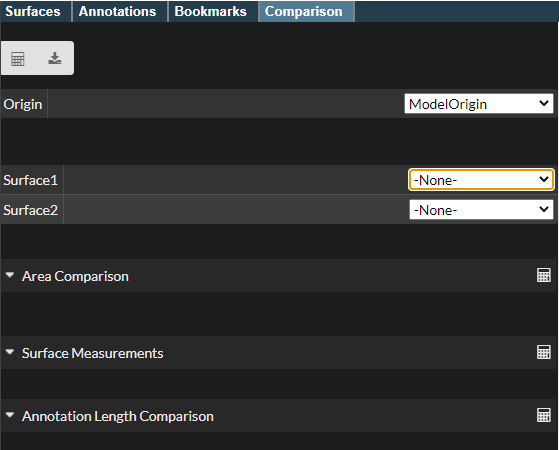
\includegraphics[width=0.6\textwidth]{pics/surfaceComparison.PNG}
	\caption[The surface comparison interface.]{The Surface Comparison Interface.}
	\label{fig:surfaceComparison}
\end{figure}

Use the drop down labelled \emph{Origin} to select which point should be used as the centre of a surface for various calculations.

In the drop down boxes labelled \emph{Surface1} and \emph{Surface2} you can select the surfaces you wish to compare. Once you have selected two surfaces, you can toggle their visibility using the \texttt{t} button on your keyboard. The calculation of surface measurements is also triggered by selecting two surfaces. You can update the measurements by clicking on the button with the calculator icon (figure \ref{surfaceComparisonAreaUpdButton.PNG}). To export all measurements click on button with the download icon (figure \ref{surfaceComparisonAreaExpButton.PNG}). The measurements will be saved in the PRo3D home directory. The full path is printed on the console when exporting.

\begin{figure}[h]
	\centering
	
\includegraphics[width=0.6\textwidth]{pics/surfaceComparisonAreaExpButton.PNG}
	\caption[The export button.]{The \emph{export} button is circled in red. Click on this button to export all listed measurements.}
	\label{surfaceComparisonAreaExpButton.PNG}
\end{figure}

\subsection{Comparing Selected Areas}

Make sure that two surfaces are loaded and selected in the \emph{Comparison} tab. In the menu bar above the 3D-View, choose \emph{Select Area} from the drop down (figure \ref{fig:surfaceComparisonAreaSelection}).

\begin{figure}[h]
	\centering
	
\includegraphics[width=0.8\textwidth]{pics/surfaceComparisonSelectArea.PNG}
	\caption[Selecting an area to compare.]{Selecting an area to compare.}
	\label{fig:surfaceComparisonAreaSelection}
\end{figure}

Hold the control key on your keyboard and click on a point on a surface to choose a location. You might need to click twice, if the 3D-View is not in focus. Once you have selected a location, a translucent sphere indicates the selected area (figure \ref{fig:surfaceComparisonAreaSphere}). You can make this sphere smaller by pressing the \emph{minus} key, bigger by pressing the \emph{plus} key on your keyboard. All vertices within a certain distances to the selected location are taken into account (in other words, the area is spherical).

\begin{figure}[h]
	\centering
	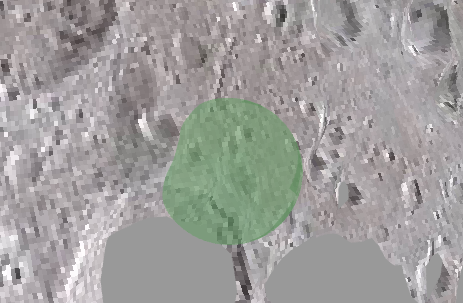
\includegraphics[width=0.6\textwidth]{pics/surfaceComparisonAreaSphere.PNG}
	\caption[A selected area.]{A selected area.}
	\label{fig:surfaceComparisonAreaSphere}
\end{figure}

All areas you have created are displayed in a list (figure \ref{fig:surfaceComparisonAreaGui}). If you wish to change the location of an area, simply delete it by clicking on the red cross and select a new location. 

\begin{figure}[h]
	\centering
	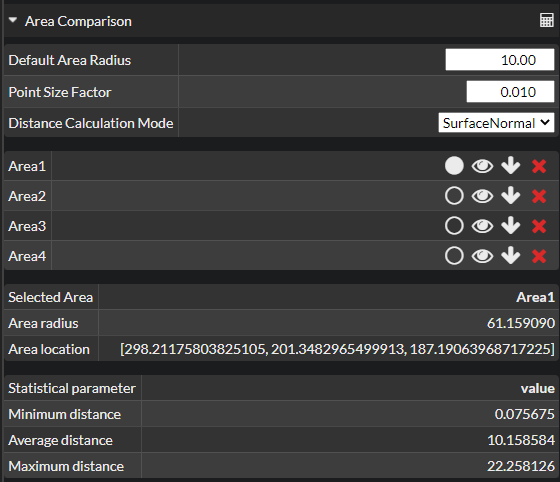
\includegraphics[width=0.6\textwidth]{pics/surfaceComparisonAreaGui.PNG}
	\caption[The interface for area comparison.]{The interface for area comparison.}
	\label{fig:surfaceComparisonAreaGui}
\end{figure}

The following settings area available for area comparison:

\begin{itemize}
	\item \textbf{Default Area Radius} The initial radius of an area when it is created. Set this according to the scale of your models.
	\item \textbf{Point Size Factor} The size of the little coloured spheres in the visualisation of differences between the two surfaces. Given an area size $a$, and a factor $f$, the size of the coloured spheres is $a * f$. Increase this factor to make the coloured spheres bigger and decrease it to make them smaller.
	\item \textbf{Distance Calculation Mode} The SurfaceNormal mode can be used for any surfaces, if in doubt use this mode. Use the Spherical Mode only for spherical surfaces. It can deal with holes in spherical surfaces, which the SurfaceNormal mode can't. \emph{Technical Note: Distances are calculated by sending rays from the vertices of one surface towards the other surface and calculating the distance between the original vertex and the intersection of the ray with the other surface. In the default mode \emph{SurfaceNormal}, the ray direction is determined by fitting a plane to the vertices in the selected area. In Spherical mode, the direction is calculated for each vertex individually based on the centre of the bounding box of the surface. For large areas on spherical surfaces this might be more suitable.}
\end{itemize}


In figure \ref{fig:surfaceComparisonAreaGui}, \emph{Area1} is selected. With the eye icon button you can set the visibility of an area. The arrow icon can be used to toggle the resolution of the vertex statistics analysis between lower and higher. This has a big effect if the two surfaces have a very different resolutions, and determines the vertices of which surface are used as a basis to calculate and visualise the differences between the two surfaces.

Once an area is to your liking, update the measurements by clicking on the calculator button (figure \ref{surfaceComparisonAreaUpdButton.PNG}). Depending on the size of the area and the resolution of the surfaces, this might take a few seconds.

\begin{figure}[h]
	\centering
	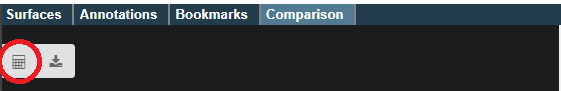
\includegraphics[width=0.6\textwidth]{pics/surfaceComparisonAreaUpdButton.PNG}
	\caption[The update button.]{The \emph{update} button is circled in red. To update all comparison calculations and visualisations click on this button.}
	\label{surfaceComparisonAreaUpdButton.PNG}
\end{figure}

\begin{figure}[h]
	\centering
	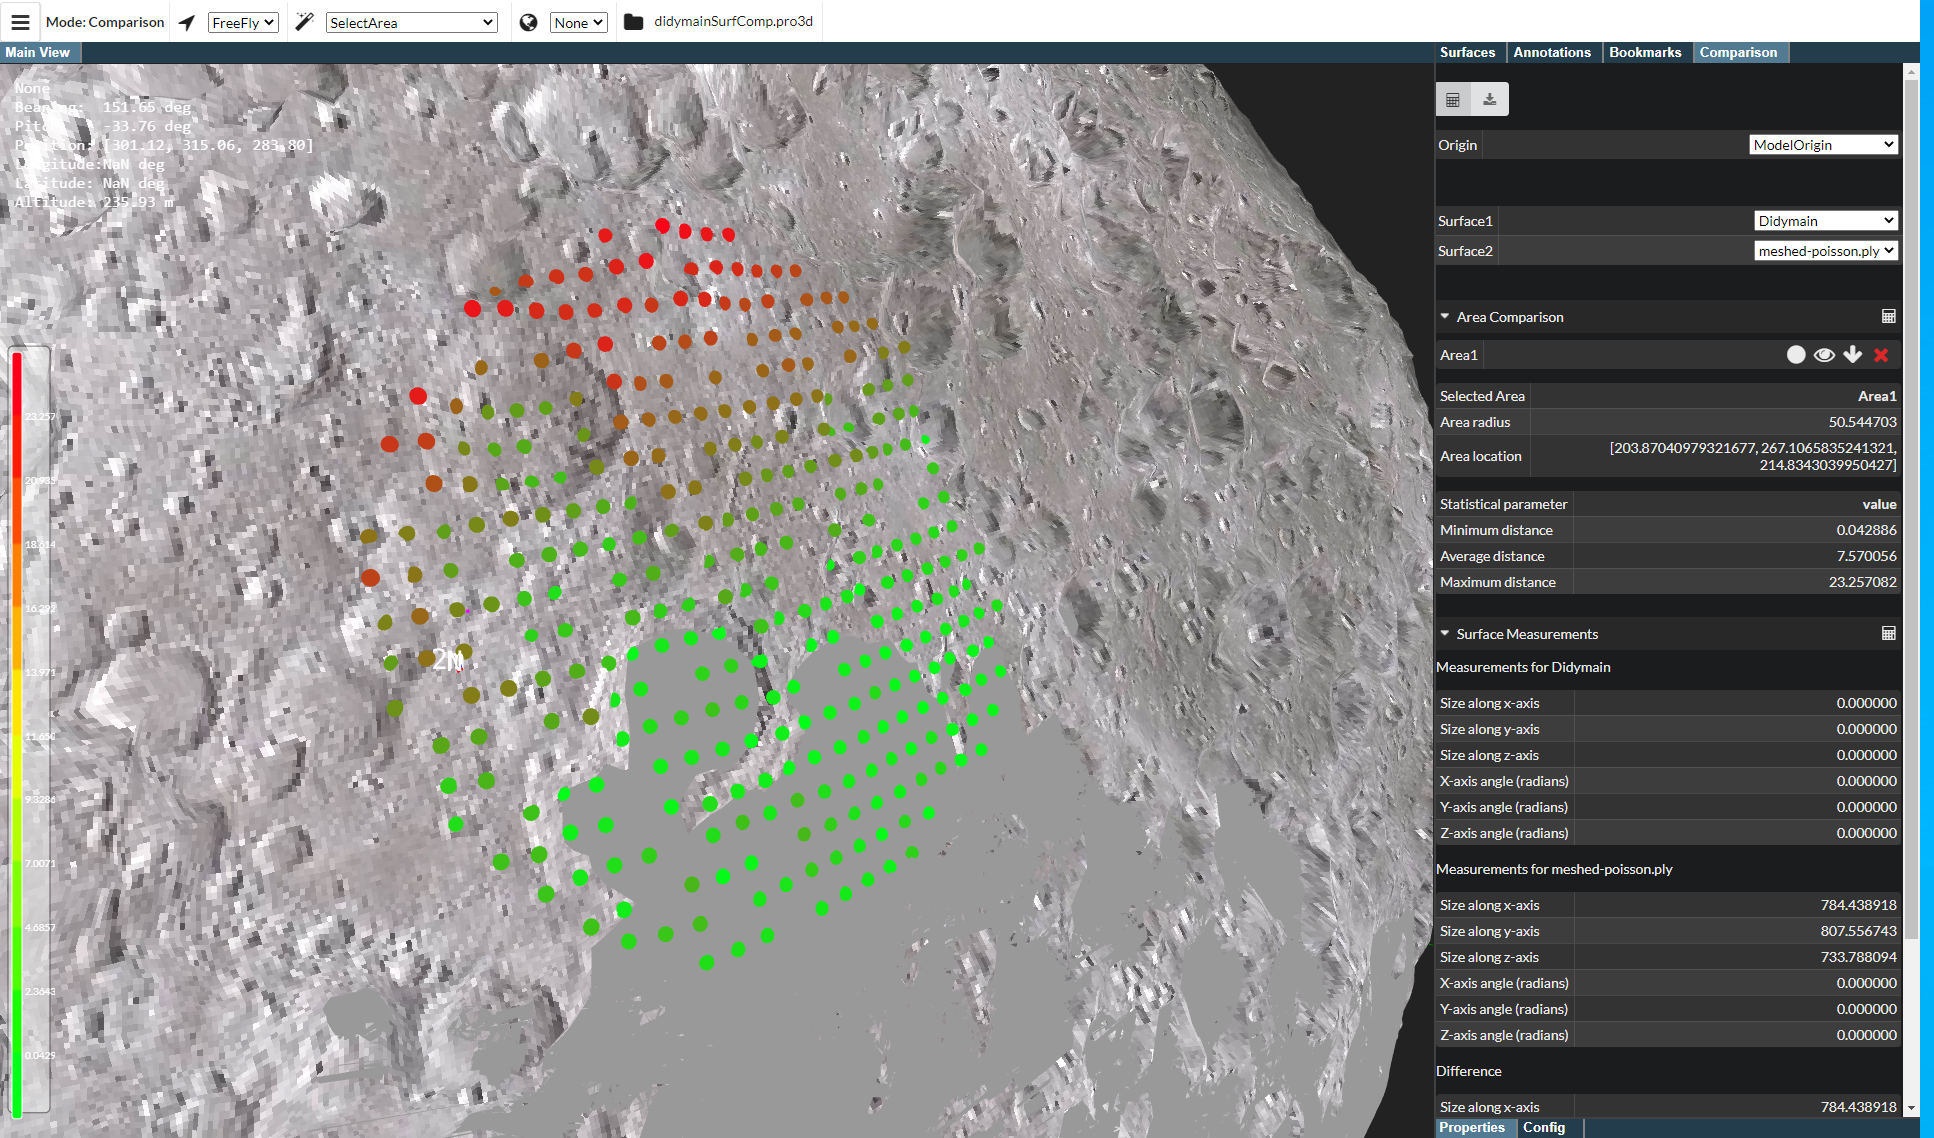
\includegraphics[width=1.0\textwidth]{pics/surfaceComparisonArea3DView1.PNG}
	\caption[Comparing an area of two surfaces.]{Comparing an area of two surfaces.}
	\label{surfaceComparisonArea3DView1.PNG}
\end{figure}

Each location that was used to calculate the distance between the two surfaces is visualised with a coloured sphere (figure \ref{surfaceComparisonArea3DView1.PNG}). The colour of the sphere encodes the distance, with red encoding large distances and green small distances. The concrete values assigned to each colour can be seen on the legend on the left. Area size, area location, and statistic parameters are displayed on the right hand side for the selected area. The legend is always valid for the selected area.

\begin{figure}[h]
	\centering
	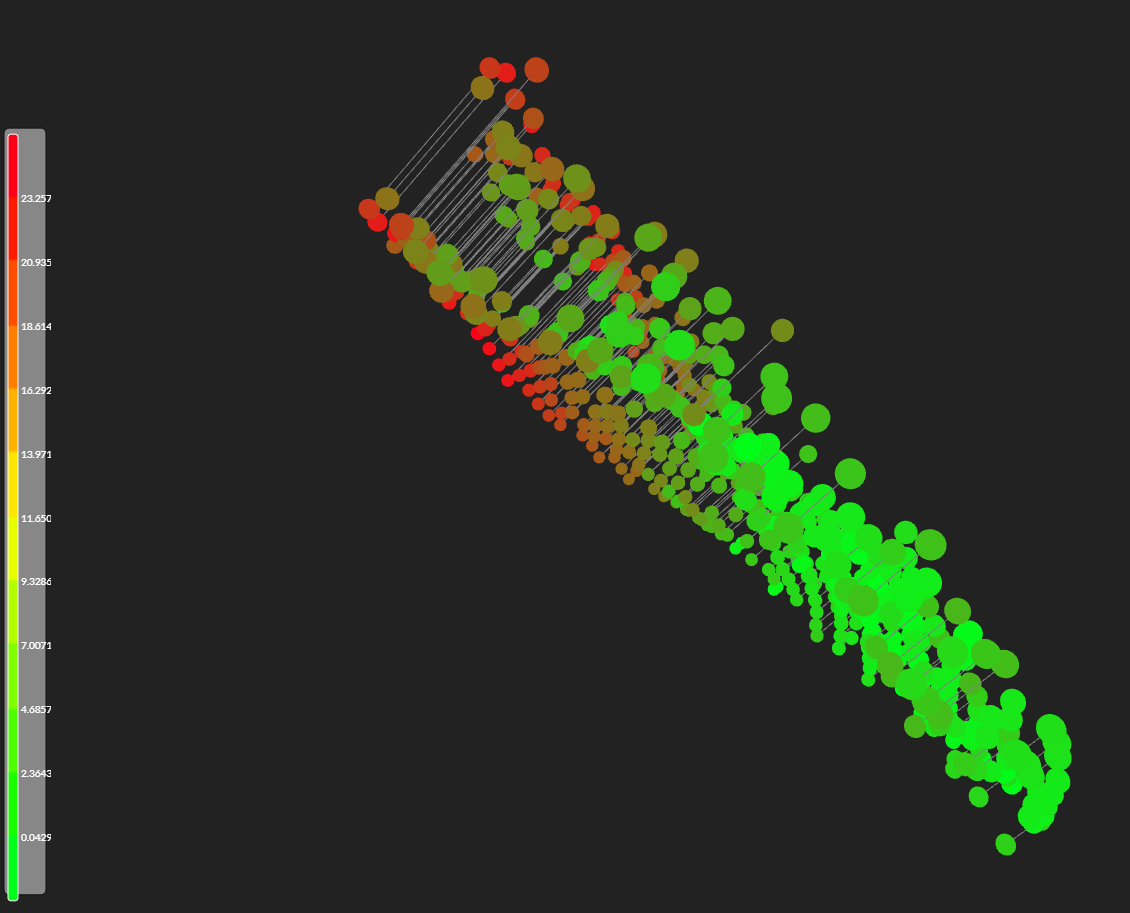
\includegraphics[width=0.8\textwidth]{pics/surfaceComparisonArea3DView2.PNG}
	\caption[Visualising the differences between two surfaces.]{Visualising the differences between two surfaces on a vertex level. The surfaces have been set to invisible.}
	\label{surfaceComparisonArea3DView2.PNG}
\end{figure}

To explore the differences between the two surfaces in more detail, set one or both areas to invisible (in the surfaces tab, use the eye icon). Figure \ref{surfaceComparisonArea3DView2.PNG} shows the difference visualisation with both areas set to invisible.

\clearpage
\subsection{Comparing Length Measurements}

To compare length measurements, create a bookmark and make sure it is selected. This bookmark can now be used as a projection point for annotations. For this, select the Bookmark projection mode for annotation drawing (figure \ref{fig:surfaceComparisonBookmarkMode}).

\begin{figure}[h]
	\centering
	
\includegraphics[width=0.7\textwidth]{pics/surfaceComparisonBookmarkMode.PNG}
	\caption[The Bookmark Projection Mode.]{The Bookmark projection mode for comparing length measurements on two surfaces. Make sure a bookmark is selected when using this mode.}
	\label{fig:surfaceComparisonBookmarkMode}
\end{figure}

Now draw one annotation on each of the two surfaces while the same bookmark is selected. Use the \texttt{t} button on your keyboard to toggle visibility between the two surfaces. Return to the comparison window and click the button with the calculator icon to update the calculations. The measurements for annotations are listed under the heading \emph{Annotation Length Comparison}.

Bookmarks can be exported and imported using the menu. Select the main menu (top left), then \emph{Bookmarks}, then \emph{Import} or \emph{Export}.
%----------------------------------------------------------------------------------------
%	Section: Keyboard Shortcuts
%----------------------------------------------------------------------------------------
%----------------------------------------------------------------------------------------
%	Section: PRo3D Command Line Interface
%----------------------------------------------------------------------------------------
\section{PRo3D Keyboard Shortcuts}


\begin{center}
	\begin{table}[h!]
		\begin{tabular}{p{0.25\linewidth} p{0.7\linewidth} }
			\textbf{Shortcut}          		 & \textbf{Description} \\
			\midrule
			f           			&  toggle linear texture magnification filtering\\
			p						&  show/hide exploration point \\
			t                       &  toggle visibility between two surfaces selected in the Comparison window
			page up/down	    	&  raise/lower navigation sensitivity\\
			ctrl s					&  save existing scene (use the menu to save a new scene) \\
			ctrl c					&  print current camera parameters in snapshot format on the command line \\
			space					&  save waypoint \\
			F1  					&  Interaction: Pick Explore Center \\
			F2 					    &  Interaction: Draw Annotation \\
			F3 						&  Interaction: Pick Annotation \\
			F4						&  Interaction: Place Coordinate System \\
			\specialrule{\lightrulewidth}{1.0pt}{4.0pt}
		\end{tabular}    
		
		\caption{A List of keyboard shortcuts in PRo3D} 
		
		\label{table:keyboardShortscuts} 
	\end{table}
\end{center}

%----------------------------------------------------------------------------------------

%----------------------------------------------------------------------------------------
%	Section: Appendix
%----------------------------------------------------------------------------------------
\section{Appendix}

\subsection{Multitexturing: Example of the currently available data} \label{multitexturingAppendix}

\lstinputlisting[language=json, label=lst:json1]{currentlyAvailableData.json}


%	END OF DOCUMENT
%----------------------------------------------------------------------------------------


\end{document}

